% Created by tikzDevice version 0.10.1 on 2017-03-15 16:22:56
% !TEX encoding = UTF-8 Unicode
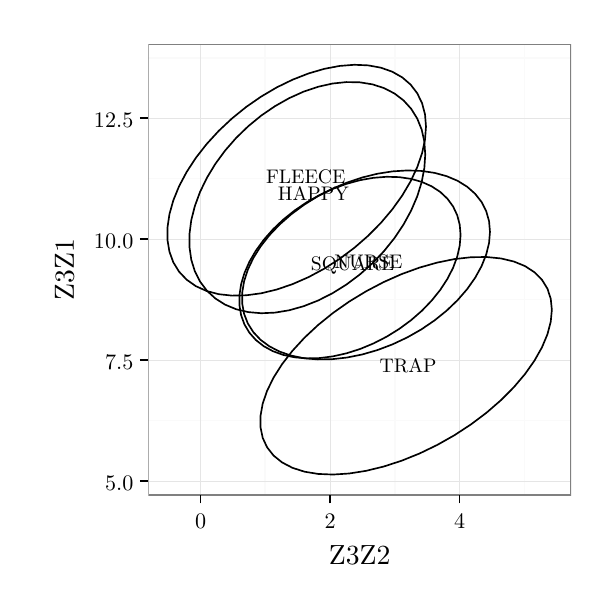
\begin{tikzpicture}[x=1pt,y=1pt]
\definecolor{fillColor}{RGB}{255,255,255}
\path[use as bounding box,fill=fillColor,fill opacity=0.00] (0,0) rectangle (202.36,202.36);
\begin{scope}
\path[clip] (  0.00,  0.00) rectangle (202.36,202.36);
\definecolor{drawColor}{RGB}{255,255,255}
\definecolor{fillColor}{RGB}{255,255,255}

\path[draw=drawColor,line width= 0.6pt,line join=round,line cap=round,fill=fillColor] (  0.00,  0.00) rectangle (202.36,202.36);
\end{scope}
\begin{scope}
\path[clip] ( 43.58, 33.48) rectangle (196.36,196.36);
\definecolor{fillColor}{RGB}{255,255,255}

\path[fill=fillColor] ( 43.58, 33.48) rectangle (196.36,196.36);
\definecolor{drawColor}{gray}{0.98}

\path[draw=drawColor,line width= 0.6pt,line join=round] ( 43.58, 60.42) --
	(196.36, 60.42);

\path[draw=drawColor,line width= 0.6pt,line join=round] ( 43.58,104.12) --
	(196.36,104.12);

\path[draw=drawColor,line width= 0.6pt,line join=round] ( 43.58,147.82) --
	(196.36,147.82);

\path[draw=drawColor,line width= 0.6pt,line join=round] ( 43.58,191.51) --
	(196.36,191.51);

\path[draw=drawColor,line width= 0.6pt,line join=round] ( 85.87, 33.48) --
	( 85.87,196.36);

\path[draw=drawColor,line width= 0.6pt,line join=round] (132.68, 33.48) --
	(132.68,196.36);

\path[draw=drawColor,line width= 0.6pt,line join=round] (179.49, 33.48) --
	(179.49,196.36);
\definecolor{drawColor}{gray}{0.90}

\path[draw=drawColor,line width= 0.2pt,line join=round] ( 43.58, 38.57) --
	(196.36, 38.57);

\path[draw=drawColor,line width= 0.2pt,line join=round] ( 43.58, 82.27) --
	(196.36, 82.27);

\path[draw=drawColor,line width= 0.2pt,line join=round] ( 43.58,125.97) --
	(196.36,125.97);

\path[draw=drawColor,line width= 0.2pt,line join=round] ( 43.58,169.67) --
	(196.36,169.67);

\path[draw=drawColor,line width= 0.2pt,line join=round] ( 62.47, 33.48) --
	( 62.47,196.36);

\path[draw=drawColor,line width= 0.2pt,line join=round] (109.28, 33.48) --
	(109.28,196.36);

\path[draw=drawColor,line width= 0.2pt,line join=round] (156.08, 33.48) --
	(156.08,196.36);
\definecolor{drawColor}{RGB}{0,0,0}

\node[text=drawColor,anchor=base,inner sep=0pt, outer sep=0pt, scale=  0.71] at (100.49,146.02) {FLEECE};

\node[text=drawColor,anchor=base,inner sep=0pt, outer sep=0pt, scale=  0.71] at (103.25,139.78) {HAPPY};

\node[text=drawColor,anchor=base,inner sep=0pt, outer sep=0pt, scale=  0.71] at (123.15,115.34) {NURSE};

\node[text=drawColor,anchor=base,inner sep=0pt, outer sep=0pt, scale=  0.71] at (117.45,114.60) {SQUARE};

\node[text=drawColor,anchor=base,inner sep=0pt, outer sep=0pt, scale=  0.71] at (137.43, 77.78) {TRAP};

\path[draw=drawColor,line width= 0.6pt,line join=round] (143.93,166.62) --
	(143.58,171.01) --
	(142.52,175.04) --
	(140.77,178.66) --
	(138.37,181.79) --
	(135.34,184.40) --
	(131.73,186.45) --
	(127.60,187.91) --
	(123.00,188.74) --
	(118.02,188.95) --
	(112.72,188.53) --
	(107.18,187.48) --
	(101.50,185.82) --
	( 95.74,183.57) --
	( 90.01,180.78) --
	( 84.39,177.47) --
	( 78.96,173.71) --
	( 73.81,169.54) --
	( 69.01,165.04) --
	( 64.64,160.27) --
	( 60.76,155.30) --
	( 57.44,150.21) --
	( 54.71,145.07) --
	( 52.63,139.96) --
	( 51.23,134.97) --
	( 50.52,130.16) --
	( 50.52,125.61) --
	( 51.23,121.39) --
	( 52.63,117.56) --
	( 54.71,114.18) --
	( 57.44,111.30) --
	( 60.76,108.96) --
	( 64.64,107.21) --
	( 69.01,106.06) --
	( 73.81,105.54) --
	( 78.96,105.65) --
	( 84.39,106.38) --
	( 90.01,107.74) --
	( 95.74,109.70) --
	(101.50,112.22) --
	(107.18,115.28) --
	(112.72,118.82) --
	(118.02,122.79) --
	(123.00,127.13) --
	(127.60,131.78) --
	(131.73,136.66) --
	(135.34,141.70) --
	(138.37,146.83) --
	(140.77,151.96) --
	(142.52,157.02) --
	(143.58,161.93) --
	(143.93,166.62);

\path[draw=drawColor,line width= 0.6pt,line join=round] (143.66,156.52) --
	(143.34,161.17) --
	(142.38,165.51) --
	(140.79,169.48) --
	(138.59,173.02) --
	(135.83,176.07) --
	(132.54,178.58) --
	(128.77,180.53) --
	(124.58,181.88) --
	(120.03,182.61) --
	(115.20,182.70) --
	(110.15,182.17) --
	(104.96,181.01) --
	( 99.71,179.24) --
	( 94.49,176.89) --
	( 89.36,173.99) --
	( 84.41,170.60) --
	( 79.71,166.75) --
	( 75.33,162.52) --
	( 71.35,157.96) --
	( 67.81,153.14) --
	( 64.78,148.13) --
	( 62.29,143.02) --
	( 60.40,137.87) --
	( 59.11,132.78) --
	( 58.47,127.80) --
	( 58.47,123.03) --
	( 59.11,118.52) --
	( 60.40,114.36) --
	( 62.29,110.60) --
	( 64.78,107.30) --
	( 67.81,104.51) --
	( 71.35,102.27) --
	( 75.33,100.62) --
	( 79.71, 99.58) --
	( 84.41, 99.17) --
	( 89.36, 99.39) --
	( 94.49,100.24) --
	( 99.71,101.71) --
	(104.96,103.77) --
	(110.15,106.40) --
	(115.20,109.55) --
	(120.03,113.18) --
	(124.58,117.22) --
	(128.77,121.63) --
	(132.54,126.33) --
	(135.83,131.25) --
	(138.59,136.32) --
	(140.79,141.46) --
	(142.38,146.59) --
	(143.34,151.64) --
	(143.66,156.52);

\path[draw=drawColor,line width= 0.6pt,line join=round] (167.05,128.59) --
	(166.72,132.43) --
	(165.70,136.03) --
	(164.03,139.34) --
	(161.72,142.30) --
	(158.82,144.87) --
	(155.36,147.02) --
	(151.40,148.70) --
	(147.00,149.90) --
	(142.22,150.59) --
	(137.14,150.77) --
	(131.83,150.43) --
	(126.38,149.58) --
	(120.86,148.22) --
	(115.37,146.39) --
	(109.98,144.11) --
	(104.78,141.41) --
	( 99.84,138.33) --
	( 95.24,134.92) --
	( 91.05,131.24) --
	( 87.33,127.34) --
	( 84.14,123.27) --
	( 81.53,119.10) --
	( 79.54,114.89) --
	( 78.20,110.71) --
	( 77.52,106.62) --
	( 77.52,102.68) --
	( 78.20, 98.96) --
	( 79.54, 95.50) --
	( 81.53, 92.35) --
	( 84.14, 89.58) --
	( 87.33, 87.22) --
	( 91.05, 85.30) --
	( 95.24, 83.86) --
	( 99.84, 82.91) --
	(104.78, 82.48) --
	(109.98, 82.56) --
	(115.37, 83.16) --
	(120.86, 84.26) --
	(126.38, 85.86) --
	(131.83, 87.92) --
	(137.14, 90.42) --
	(142.22, 93.31) --
	(147.00, 96.56) --
	(151.40,100.11) --
	(155.36,103.91) --
	(158.82,107.90) --
	(161.72,112.03) --
	(164.03,116.22) --
	(165.70,120.42) --
	(166.72,124.57) --
	(167.05,128.59);

\path[draw=drawColor,line width= 0.6pt,line join=round] (156.43,127.47) --
	(156.12,131.14) --
	(155.22,134.58) --
	(153.73,137.74) --
	(151.67,140.56) --
	(149.08,143.00) --
	(145.99,145.02) --
	(142.46,146.61) --
	(138.53,147.72) --
	(134.26,148.35) --
	(129.73,148.48) --
	(124.99,148.11) --
	(120.13,147.26) --
	(115.21,145.92) --
	(110.31,144.12) --
	(105.50,141.90) --
	(100.85,139.27) --
	( 96.45,136.29) --
	( 92.34,133.00) --
	( 88.60,129.44) --
	( 85.29,125.67) --
	( 82.44,121.76) --
	( 80.11,117.75) --
	( 78.33,113.71) --
	( 77.13,109.69) --
	( 76.53,105.77) --
	( 76.53,102.00) --
	( 77.13, 98.44) --
	( 78.33, 95.13) --
	( 80.11, 92.14) --
	( 82.44, 89.51) --
	( 85.29, 87.27) --
	( 88.60, 85.46) --
	( 92.34, 84.11) --
	( 96.45, 83.24) --
	(100.85, 82.86) --
	(105.50, 82.97) --
	(110.31, 83.59) --
	(115.21, 84.69) --
	(120.13, 86.25) --
	(124.99, 88.27) --
	(129.73, 90.70) --
	(134.26, 93.51) --
	(138.53, 96.65) --
	(142.46,100.08) --
	(145.99,103.75) --
	(149.08,107.60) --
	(151.67,111.57) --
	(153.73,115.61) --
	(155.22,119.64) --
	(156.12,123.61) --
	(156.43,127.47);

\path[draw=drawColor,line width= 0.6pt,line join=round] (189.41,100.42) --
	(189.01,104.41) --
	(187.82,108.04) --
	(185.85,111.24) --
	(183.14,113.97) --
	(179.73,116.20) --
	(175.66,117.87) --
	(171.00,118.97) --
	(165.83,119.49) --
	(160.21,119.41) --
	(154.24,118.74) --
	(148.00,117.48) --
	(141.59,115.66) --
	(135.10,113.30) --
	(128.64,110.43) --
	(122.31,107.11) --
	(116.19,103.39) --
	(110.38, 99.31) --
	(104.97, 94.94) --
	(100.05, 90.35) --
	( 95.68, 85.60) --
	( 91.93, 80.77) --
	( 88.86, 75.93) --
	( 86.52, 71.16) --
	( 84.93, 66.53) --
	( 84.14, 62.10) --
	( 84.14, 57.95) --
	( 84.93, 54.13) --
	( 86.52, 50.71) --
	( 88.86, 47.74) --
	( 91.93, 45.26) --
	( 95.68, 43.31) --
	(100.05, 41.91) --
	(104.97, 41.10) --
	(110.38, 40.88) --
	(116.19, 41.26) --
	(122.31, 42.23) --
	(128.64, 43.77) --
	(135.10, 45.87) --
	(141.59, 48.48) --
	(148.00, 51.58) --
	(154.24, 55.11) --
	(160.21, 59.02) --
	(165.83, 63.25) --
	(171.00, 67.74) --
	(175.66, 72.42) --
	(179.73, 77.22) --
	(183.14, 82.06) --
	(185.85, 86.87) --
	(187.82, 91.58) --
	(189.01, 96.12) --
	(189.41,100.42);
\definecolor{drawColor}{gray}{0.50}

\path[draw=drawColor,line width= 0.6pt,line join=round,line cap=round] ( 43.58, 33.48) rectangle (196.36,196.36);
\end{scope}
\begin{scope}
\path[clip] (  0.00,  0.00) rectangle (202.36,202.36);
\definecolor{drawColor}{RGB}{0,0,0}

\node[text=drawColor,anchor=base east,inner sep=0pt, outer sep=0pt, scale=  0.80] at ( 38.18, 35.26) {5.0};

\node[text=drawColor,anchor=base east,inner sep=0pt, outer sep=0pt, scale=  0.80] at ( 38.18, 78.96) {7.5};

\node[text=drawColor,anchor=base east,inner sep=0pt, outer sep=0pt, scale=  0.80] at ( 38.18,122.66) {10.0};

\node[text=drawColor,anchor=base east,inner sep=0pt, outer sep=0pt, scale=  0.80] at ( 38.18,166.36) {12.5};
\end{scope}
\begin{scope}
\path[clip] (  0.00,  0.00) rectangle (202.36,202.36);
\definecolor{drawColor}{RGB}{0,0,0}

\path[draw=drawColor,line width= 0.6pt,line join=round] ( 40.58, 38.57) --
	( 43.58, 38.57);

\path[draw=drawColor,line width= 0.6pt,line join=round] ( 40.58, 82.27) --
	( 43.58, 82.27);

\path[draw=drawColor,line width= 0.6pt,line join=round] ( 40.58,125.97) --
	( 43.58,125.97);

\path[draw=drawColor,line width= 0.6pt,line join=round] ( 40.58,169.67) --
	( 43.58,169.67);
\end{scope}
\begin{scope}
\path[clip] (  0.00,  0.00) rectangle (202.36,202.36);
\definecolor{drawColor}{RGB}{0,0,0}

\path[draw=drawColor,line width= 0.6pt,line join=round] ( 62.47, 30.48) --
	( 62.47, 33.48);

\path[draw=drawColor,line width= 0.6pt,line join=round] (109.28, 30.48) --
	(109.28, 33.48);

\path[draw=drawColor,line width= 0.6pt,line join=round] (156.08, 30.48) --
	(156.08, 33.48);
\end{scope}
\begin{scope}
\path[clip] (  0.00,  0.00) rectangle (202.36,202.36);
\definecolor{drawColor}{RGB}{0,0,0}

\node[text=drawColor,anchor=base,inner sep=0pt, outer sep=0pt, scale=  0.80] at ( 62.47, 21.47) {0};

\node[text=drawColor,anchor=base,inner sep=0pt, outer sep=0pt, scale=  0.80] at (109.28, 21.47) {2};

\node[text=drawColor,anchor=base,inner sep=0pt, outer sep=0pt, scale=  0.80] at (156.08, 21.47) {4};
\end{scope}
\begin{scope}
\path[clip] (  0.00,  0.00) rectangle (202.36,202.36);
\definecolor{drawColor}{RGB}{0,0,0}

\node[text=drawColor,anchor=base,inner sep=0pt, outer sep=0pt, scale=  1.00] at (119.97,  8.40) {Z3Z2};
\end{scope}
\begin{scope}
\path[clip] (  0.00,  0.00) rectangle (202.36,202.36);
\definecolor{drawColor}{RGB}{0,0,0}

\node[text=drawColor,rotate= 90.00,anchor=base,inner sep=0pt, outer sep=0pt, scale=  1.00] at ( 16.67,114.92) {Z3Z1};
\end{scope}
\end{tikzpicture}
